\documentclass[a4paper,12pt]{article}
\usepackage[utf8]{inputenc}

\usepackage[french]{babel}
\usepackage{enumitem}
\usepackage{graphicx}
\usepackage{multirow}
\usepackage{hyperref}
\usepackage{pgf-pie}
\usepackage{tikz}
\usepackage{fancyhdr}

\pagestyle{fancy}
\frenchbsetup{StandardLists=true}

\title{Présentation des langages de programmation}
\author{Wikipédia, Xavier Dufillon \& Gaëtan Croquefer}

\lfoot{Wikipédia}
\rfoot{\today}

\begin{document}

\maketitle
\newpage

\renewcommand{\contentsname}{Sommaire}
\tableofcontents
\newpage
\listoffigures
\newpage

\setlength{\parindent}{0em}
\section{Résumé}

En informatique, un langage de programmation est une notation conventionnelle destinée à formuler des algorithmes et produire des programmes informatiques qui les appliquent. D'une manière similaire à une langue naturelle, un langage de programmation est composé d'un alphabet, d'un vocabulaire, de règles de grammaire et de significations.\cite{maurizio} \cite{kenneth}\\
Les langages de programmation permettent de décrire d'une part les structures des données qui seront manipulées par l'appareil informatique, et d'autre part d'indiquer comment sont effectuées les manipulations, selon quels algorithmes. Ils servent de moyens de communication par lesquels le programmeur communique avec l'ordinateur, mais aussi avec d'autres programmeurs ; les programmes étant d'ordinaire écrits, lus, compris et modifiés par une équipe de programmeurs.\cite{william}\\
Un langage de programmation est mis en œuvre par un traducteur automatique : compilateur ou interpréteur. Un compilateur est un programme informatique qui transforme dans un premier temps un code source écrit dans un langage de programmation donné en un code cible qui pourra être directement exécuté par un ordinateur, à savoir un programme en langage machine ou en code intermédiaire\cite{kenneth}, tandis que l'interpréteur réalise cette traduction « à la volée ».\\
Les langages de programmation offrent différentes possibilités d'abstraction, et une notation proche de l'algèbre, permettant de décrire de manière concise et facile à saisir les opérations de manipulation de données et l'évolution du déroulement du programme en fonction des situations. La possibilité d'écriture abstraite libère l'esprit du programmeur d'un travail superflu, notamment de prise en compte des spécificités du matériel informatique, et lui permet ainsi de se concentrer sur des problèmes plus avancés.\cite{kenneth}\\
Chaque langage de programmation supporte un ou plusieurs styles de programmation – paradigmes. Les notions propres au paradigme font partie du langage de programmation, permettant au programmeur d'exprimer dans le langage de programmation une solution qui a été imaginée selon ce paradigme.
Les premiers langages de programmation ont été créés dans les années 1950. De nombreux concepts de l'informatique ont été lancés par un langage, avant d'être améliorés et étendus dans les langages suivants. La plupart du temps la conception d'un langage de programmation a été fortement influencée par l'expérience acquise avec les langages précédents.\cite{watt}

\section{Définition}

Un langage de programmation est construit à partir d'une grammaire formelle, qui inclut des symboles et des règles syntaxiques, auxquels on associe des règles sémantiques. Ces éléments sont plus ou moins complexes selon la capacité du langage. Les modes de fonctionnement et de définition de la complexité d'un langage de programmation sont généralement déterminés par leur appartenance à l'un des degrés de la Hiérarchie de Chomsky.

Sous un angle théorique, tout langage informatique peut être qualifié de langage de programmation s'il est Turing-complet c'est-à-dire qu'il permet de représenter toutes les fonctions calculables au sens de Turing et Church (en admettant néanmoins pour exception à la théorie que la mémoire des ordinateurs n'est pas un espace infini)\cite{lando}.

\begin{itemize}[label=\textbullet]

\setlength{\itemindent}{-1.5em}

\item Les règles de syntaxe
\newline Définies par une grammaire formelle, elles régissent les différentes manières dont les éléments du langage peuvent être combinés pour obtenir des programmes\cite{kenneth}. La ponctuation (par exemple l'apposition d'un symbole ; en fin de ligne d'instruction d'un programme) relève de la syntaxe.

\item Le vocabulaire
\newline Parmi les éléments du langage, le vocabulaire représente l'ensemble des instructions construites d’après des symboles. L'instruction peut être mnémotechnique ou uniquement symbolique comme quand elle est représentée par des symboles d'opérations tels que des opérateurs arithmétiques (« + » et « - ») ou booléens (\&\& pour le et logique par exemple). On parle aussi parfois de mot clé pour désigner une instruction (par abus de langage car le concept de mot clé ne recouvre pas celui des symboles qui font pourtant eux aussi partie du vocabulaire).

\item La sémantique
\newline Les règles de sémantique définissent le sens de chacune des phrases qui peuvent être construites dans le langage, en particulier quels seront les effets de la phrase lors de l'exécution du programme\cite{kenneth}. La science l'étudiant est la sémantique des langages de programmation.

\item L'alphabet
\newline L'alphabet des langages de programmation est basé sur les normes courantes comme ASCII, qui comporte les lettres de A à Z sans accent, des chiffres et des symboles\cite{seema}, ou Unicode pour la plupart des langages modernes (dans lesquels l'utilisation se limite en général aux chaînes de caractères littérales et aux commentaires, avec quelques exceptions notables comme C\# qui autorisent également les identifiants unicode).
\newline La plupart des langages de programmation peuvent prévoir des éléments de structure complémentaires, des méthodes procédurales, et des définitions temporaires et variables et des identifiants:

\item Les commentaires
\newline Les commentaires sont des textes qui ne seront pas traduits. Ils peuvent être ajoutés dans les programmes pour y laisser des explications. Les commentaires sont délimités par des marques qui diffèrent d'un langage de programmation à l'autre tel que « -- », « /* » ou « // »\cite{seema}.

\item Les identifiants
\newline Les éléments constitutifs du programme, tels que les variables, les procédures, ou les types servent à organiser le programme et son fonctionnement. On peut ainsi, par exemple, diviser un programme en fonctions, ou lui donner une structure par objets : ces éléments de structure sont définis par des identifiants ou des procédures par mot clé selon le langage.

\end{itemize}

\section{Utilisation}

Un langage de programmation offre un cadre pour élaborer des algorithmes et exprimer des diagrammes de flux\cite{itl}\cite{seema}. Il permet en particulier de décrire les structures des données qui seront manipulées par l'appareil informatique et quelles seront les manipulations. Un langage de programmation sert de moyen de communication avec l'ordinateur mais aussi entre programmeurs : les programmes étant d'ordinaire écrits, lus et modifiés par une équipe de programmeurs\cite{william}.

Un langage de programmation offre un ensemble de notions qui peuvent être utilisées comme primitives pour développer des algorithmes. Les programmeurs apprécient que le langage soit clair, simple, et unifié, qu'il y ait un minimum de notions qui peuvent être combinées selon des règles simples et régulières. Les qualités d'un langage de programmation influent sur la facilité avec laquelle les programmes pourront être écrits, testés, puis plus tard compris et modifiés\cite{seema}.

Les langages de programmation offrent différentes possibilités d'abstraction, et une notation proche de l'algèbre, permettant de décrire de manière concise et facile à saisir les opérations de manipulation de données et l'évolution du déroulement du programme en fonction des situations. Cette possibilité d'écriture abstraite libère l'esprit du programmeur d'un travail superflu, et lui permet de se concentrer sur des problèmes plus avancés\cite{kenneth}.

La facilité d'utilisation, la portabilité et la clarté sont des qualités appréciées des langages de programmation. La facilité d'utilisation, qui dépend de la syntaxe, du vocabulaire et des symboles, influence la lisibilité des programmes écrits dans ce langage et la durée d'apprentissage. La portabilité permet à un programme écrit pour être exécuté par une plateforme informatique donnée (un système d'exploitation) d'être transféré en vue d'être exécuté sur une autre plateforme\cite{itl}.

Les programmeurs apprécient que la syntaxe permette d'exprimer la structure logique inhérente au programme. Un des soucis en programmation est d'éviter des pannes, qu'il soit possible de les détecter, les éviter et les rectifier; ceci est rendu possible par des mécanismes internes des langages de programmation. Des vérifications implicites sont parfois effectuées en vue de déceler des problèmes\cite{itl}.

Les programmeurs apprécient qu'un langage de programmation soit en ligne avec les bonnes pratiques de programmation et d'ingénierie, qu'il encourage la structuration du programme, facilite la maintenance des programmes et qu'il dissuade voire interdise les mauvaises pratiques\cite{itl}. L'utilisation de l'instruction goto, par exemple, qui existe depuis les premiers langages de programmation, est considérée comme une mauvaise pratique. Son utilisation est déconseillée, voire impossible dans les langages de programmation récents\cite{barlow}.

L'alignement sur les standards industriels, la possibilité d'utiliser des fonctionnalités écrites dans un autre langage de programmation et l'exécution simultanée de plusieurs threads sont des possibilités appréciées des langages de programmation\cite{itl}.

\subsection{Notions courantes}

Un langage de programmation permet de décrire les structures des données qui seront manipulées par l'appareil informatique et quelles seront les manipulations. Il offre un ensemble de notions telles que les instructions, les variables, les types, et les procédures, qui peuvent être utilisées comme primitives pour développer des algorithmes\cite{thakare}.

\begin{itemize}[label=\textbullet]

\setlength{\itemindent}{-1.5em}

\item Une instruction :
\newline Un ordre donné à un ordinateur\cite{ada}.

\item Une variable :
\newline Un nom utilisé dans un programme pour faire référence à une donnée manipulée par programme.

\item Une constante : 
\newline Un nom utilisé pour faire référence à une valeur permanente.

\item Une expression littérale :
\newline Une valeur mentionnée en toutes lettres dans le programme\cite{thakare}.

\item Un type :
\newline Chaque donnée a une classification, celle-ci influe sur la plage de valeurs possibles, les opérations qui peuvent être effectuées, et la représentation de la donnée sous forme de bits\cite{thakare}. Chaque langage de programmation offre une gamme de types primitifs, incorporés dans le langage. Certains langages offrent la possibilité de créer des nouveaux types.		
\newline Les types de données primitifs courants sont les nombres entiers, les nombres réels, le booléen, les chaînes de caractères et les pointeurs.
\newline Plus précisément, le type booléen est un type qui n'a que deux valeurs, vrai et faux, tandis que le type pointeur : une référence à une donnée, qui se trouve quelque part en mémoire\cite{thakare}.

\item Une structure de données
\newline Une manière caractéristique d'organiser un ensemble de données en mémoire, qui influe sur les algorithmes utilisés pour les manipuler. Les structures courantes sont les tableaux, les enregistrements, les listes, les piles et les arbres\cite{krishnamurthy}.

\item Une déclaration
\newline Une phrase de programme qui sert à renseigner au traducteur (compilateur, interpréteur...) les noms et les caractéristiques des éléments du programme tels que des variables, des procédures, de types\cite{william}...
\newline Des vérifications sont effectuées au moment de la compilation, ou au moment de l'exécution du programme, pour assurer que les opérations du programme sont possibles avec les types de données qui sont utilisés. Dans un langage fortement typé, chaque élément du programme a un type unique, connu et vérifié au moment de la compilation, ce qui permet de déceler des erreurs avant d'exécuter le programme\cite{william}.

\item Les procédures, fonctions, méthodes
\newline Divers langages de programmation offrent la possibilité d'isoler un fragment de programme, et d'en faire une opération générale, paramétrable, susceptible d'être utilisée de façon répétée. Ces fragments sont appelés procédures, fonctions ou méthodes, selon le paradigme.

\item Les modules
\newline Les langages de programmation peuvent également offrir la possibilité de découper un programme en plusieurs pièces appelées modules, chacune ayant un rôle déterminé, puis de combiner les pièces\cite{william}.
\newline Les notions de procédure et de module sont destinées à faciliter la création de programmes complexes et volumineux en assistant la prise en charge de cette complexité. Ces fonctions permettent en particulier la modularité et l'abstraction\cite{william}.

\end{itemize}

\section{Paradigmes}

Un paradigme est un style de programmation\cite{kumar}. Chaque paradigme amène une technique différente de programmation; une fois qu'une solution a été imaginée par le programmeur selon un certain paradigme, un langage de programmation qui suit ce paradigme permettra de l'exprimer\cite{jana}. Impératif, déclaratif, fonctionnel, logique, orienté objet, concurrent, visuel, événementiel, et basé web sont des paradigme de programmation\cite{kumar}. Chaque langage de programmation reflète un ou plusieurs paradigmes, apportant un ensemble de notions qui peuvent être utilisées pour exprimer une solution à un problème de programmation\cite{jana}. Au cours de l'histoire, les scientifiques et les programmeurs ont identifié les avantages et les limitations d'un style de programmation et apporté de nouveaux styles\cite{kumar}. Les langages de programmation contemporains de 2013 permettent typiquement d'adopter plusieurs styles de programmation\cite{kumar}. Voir \hyperref[paradigme]{Fig.1} pour une vue d'ensemble des différents paradigmes existants.

\subsection{Impératif (ou procédural)}

Le paradigme impératif ou procédural est basé sur le principe de l'exécution étape par étape des instructions tout comme on réalise une recette de cuisine. Il est basé sur le principe de la machine de Von Neumann. Un ensemble d'instructions de contrôle de flux d'exécution permet de contrôler l'ordre dans lequel sont exécutées les instructions qui décrivent les étapes. L'abstraction est réalisée à l'aide de procédures auxquelles sont transmises des données. Il existe une procédure principale, qui est la première à être exécutée, et qui peut faire appel à d'autre procédures spécialisées pour effectuer certaines tâches (commande d'appareil, calculs, etc.). Le C, le Pascal, le Fortran et le COBOL sont des exemples de langage de programmation qui implémentent le paradigme impératif\cite{jana}.

\subsection{Déclaratif}

Les deux paradigmes déclaratifs sont: fonctionnel et logique. En paradigme fonctionnel le programmeur décrit des fonctions mathématiques. En paradigme logique il décrit des prédicats : une déclaration qui peut être vraie ou fausse\cite{kumar}. Une machine abstraite effectue ensuite les opérations nécessaires pour calculer le résultat de chaque fonction et chaque prédicat. Dans ce paradigme une variable contient le résultat d'un calcul et ne peut pas être modifiée par assignation\cite{kumar}.

\subsubsection{Fonctionnel}

Le paradigme fonctionnel est basé sur l'idée d'évaluer une formule, et d'utiliser le résultat pour autre chose, selon le modèle du lambda-calcul. Tous les traitements sont faits en évaluant des expressions et en faisant appel à des fonctions, et l'exécution étape par étape n'est pas possible dans le paradigme fonctionnel. Le résultat d'un calcul sert de matière première pour le calcul suivant, et ainsi de suite, jusqu'à ce que toutes les fonctions aient produit un résultat\cite{jana}. Le paradigme fonctionnel a été introduit par le langage Lisp à la fin des années 1960. En 2013 des langages tels que Ruby et Scala supportent plusieurs styles dont le paradigme fonctionnel\cite{kumar}.

\subsubsection{Logique}

Le paradigme logique est basé sur l'idée de répondre à une question par des recherches sur un ensemble, en utilisant des axiomes, des demandes et des règles de déduction. L'exécution d'un programme est une cascade de recherches de données dans un ensemble, en faisant usage de règles de déduction. Les données obtenues, et associées à un autre ensemble de règles peuvent alors être utilisées dans le cadre d'une autre recherche. L'exécution du programme se fait par évaluation, le système effectue une recherche de toutes les affirmations qui, par déduction, correspondent à au moins un élément de l'ensemble. Le programmeur exprime les règles, et le système pilote le processus\cite{jana}. Le paradigme logique a été introduit par le langage Prolog en 1970\cite{kumar}.

\subsection{Orienté objet}

Le paradigme orienté objet est destiné à faciliter le découpage d'un grand programme en plusieurs modules isolés les uns des autres. Il introduit les notions d'objet et d'héritage. Un objet contient les variables et les fonctions en rapport avec un sujet. Les variables peuvent être privées, c'est-à-dire qu'elles peuvent être manipulées uniquement par l'objet qui les contient. Un objet contient implicitement les variables et les fonctions de ses ancêtres, et cet héritage aide à réutiliser du code\cite{kumar}. Le paradigme orienté objet permet d'associer fortement les données avec les procédures\cite{jana}. Il a été introduit par le langage Simula dans les années 1960, et est devenu populaire dans les années 1980, quand l'augmentation de la puissance de calcul des ordinateurs a permis d'exécuter des grands programmes\cite{kumar}. Divers langages de programmation ont été enrichis en vue de permettre la programmation orientée objet; c'est le cas de C++ dérivé du langage C. Simula, Smalltalk, C++ , Swift et Java sont des langages de programmation en paradigme orienté objet\cite{jana}.
\subsection{Concurrent}

En paradigme concurrent un programme peut effectuer plusieurs tâches en même temps. Ce paradigme introduit les notions de thread, d'attente active et d'appel de fonction à distance\cite{kumar}. Ces notions ont été introduites dans les années 1980 lorsque, à la suite de l'évolution technologique, un ordinateur est devenu une machine comportant plusieurs processeurs et capable d'effectuer plusieurs tâches simultanément. Les langages de programmation contemporains de 2013 tels que C++ et Java sont adaptés aux processeurs multicore et permettent de créer et manipuler des threads\cite{kumar}. Plus récemment, on a vu apparaître des langages plus modernes intégralement orientés vers la gestion de la concurrence, comme le langage Go.

\subsection{Visuel}

Dans la grande majorité des langages de programmation, le code source est un texte. Ce qui rend difficile d'exprimer des objets en deux dimensions\cite{kumar}. Un langage de programmation tel que Delphi ou C\# permet de manipuler des objets par glisser-déposer et le dessin ainsi obtenu est ensuite traduit en une représentation textuelle orientée objet et événementielle. Le paradigme visuel a été introduit à la fin des années 1980 par le langage Smalltalk, dans le but de faciliter la programmation des interfaces graphiques\cite{kumar}.

\subsection{Événementiel}

Alors qu'un programme interactif pose une question et effectue des actions en fonction de la réponse, en style événementiel le programme n'attend rien et est exécuté lorsque quelque chose s'est passé\cite{kumar}. Par exemple, l'utilisateur déplace la souris ou presse sur un bouton. Dans ce paradigme, la programmation consiste à décrire les actions à prendre en réponse aux événements. Et une action peut en cascade déclencher une autre action correspondant à un autre événement\cite{kumar}. Le paradigme événementiel a été introduit par le langage Simula dans les années 1970. Il est devenu populaire à la suite de l'avènement des interfaces graphiques et des applications web\cite{kumar}.

\subsection{Basé web}

Avec l’avènement de l'Internet dans les années 1990, les données, les images ainsi que le code s'échangent entre ordinateurs. Si un résultat est demandé à un ordinateur, celui-ci peut exécuter le programme nécessaire, et envoyer le résultat. Il peut également envoyer le code nécessaire à l'ordinateur client pour qu'il calcule le résultat lui-même\cite{kumar}. Le programme est rarement traduit en langage machine, mais plutôt interprété ou traduit en une forme intermédiaire, le bytecode, qui sera exécuté par une machine virtuelle, ou traduit en langage machine au moment de l'exécution (just-in-time). Java, PHP et Javascript sont des langages de programmation basée web\cite{kumar}.

\begin{itemize}[label=\textbullet]

\setlength{\itemindent}{-1.5em}

\item Mise en œuvre
\newline L'utilisation d'un langage est rendue possible par un traducteur automatique. Un programme qui prend un texte écrit dans ce langage pour en faire quelque chose, en général soit :

\item Un compilateur
\newline Un programme qui traduit le texte dans un langage qui permettra son exécution, tel le langage machine, le bytecode ou le langage assembleur.

\item Un interpréteur
\newline Un programme qui exécute les instructions demandées. Il joue le même rôle qu'une machine qui reconnaîtrait ce langage.

\item Langage machine
\newline Chaque appareil informatique a un ensemble d'instructions qui peuvent être utilisées pour effectuer des opérations. Les instructions permettent d'effectuer des calculs arithmétiques ou logiques, déplacer ou copier des données, ou bifurquer vers l'exécution d'autres instructions. Ces instructions sont enregistrées sous forme de séquences de bits, où chaque séquence correspond au code de l'opération à effectuer et aux opérandes, c'est-à-dire aux données concernées ; c'est le langage machine\cite{godse}.

\end{itemize}

La traduction s'effectue en plusieurs étapes. En premier lieu, le traducteur effectue une analyse lexicale où il identifie les éléments du langage utilisés dans le programme. Dans l'étape suivante, l'analyse syntaxique, le traducteur construit un diagramme en arbre qui reflète la manière dont les éléments du langage ont été combinés dans le programme, pour former des instructions. Puis lors de l'analyse sémantique le traducteur détermine s'il est possible de réaliser l'opération, et les instructions qui seront nécessaires dans le langage cible\cite{dhamdhere}.

Dans le langage de programmation assembleur, des mots aide-mémoire (mnémonique) sont utilisés pour référer aux instructions de la machine. Les instructions diffèrent en fonction des constructeurs et il en va de même pour les mnémoniques. Un programme assembleur traduit chaque mnémonique en la séquence de bits correspondante\cite{tmh}.

Les langages de programmation fonctionnent souvent à l'aide d'un runtime.

\begin{itemize}[label=\textbullet]

\setlength{\itemindent}{-1.5em}

\item Un runtime
\newline Un runtime (traduction: exécuteur) est un ensemble de bibliothèques logicielles qui mettent en œuvre le langage de programmation, permettant d'effectuer des opérations simples telles que copier des données, voire les opérations beaucoup plus complexes\cite{scott}.

\end{itemize}

Lors de la traduction d'un programme vers le langage machine, les opérations simples sont traduites en les instructions correspondantes en langage machine tandis que les opérations complexes sont traduites en des utilisations des fonctions du runtime. Dans certains langages de programmation, la totalité des instructions sont traduites en des utilisations du runtime\cite{scott} qui sert alors d'intermédiaire entre les possibilités offertes par la plateforme informatique et les constructions propre au langage de programmation\cite{griffiths}.

Chaque langage de programmation a une manière conventionnelle de traduire l'exécution de procédures ou de fonctions, de placer les variables en mémoire et de transmettre des paramètres. Ces conventions sont appliquées par le runtime\cite{raghavan}. Les runtime servent également à mettre en œuvre certaines fonctionnalités avancées des langages de programmation telles que le ramasse-miettes, ou la réflexion\cite{scott}.

Les langages de programmation sont couramment auto-implémentés, c'est-à-dire que le compilateur pour ce langage de programmation est mis en œuvre dans le langage lui-même. Exemple : un compilateur pour le langage Pascal peut être écrit en langage Pascal\cite{diomidis}.

\subsection{Fonctionnalités avancées}

Les fonctionnalités avancées telles que le ramasse-miettes (anglais garbage collector), la manipulation des exceptions, des événements, ou des threads, ainsi que la liaison tardive et la réflexion sont mises en œuvre par les runtime des langages de programmation\cite{scott}.

\begin{itemize}[label=\textbullet]

\setlength{\itemindent}{-1.5em}

\item Un ramasse-miettes
\newline Un mécanisme qui supprime les variables inutilisées et libère l'espace mémoire qui leur avait été réservé\cite{chris}.

\item Une exception
\newline Un fait inattendu, souvent accidentel, entraîne l'échec du déroulement normal du programme, et ce fait exceptionnel doit être pris en charge par le programme avant de pouvoir continuer. Certains langages de programmation permettent de provoquer délibérément l'arrêt du déroulement normal du programme\cite{friesen}.

\item Un événement
\newline Une procédure qui va être exécutée lorsqu'une condition particulière est rencontrée. les événements sont notamment utilisés pour mettre en œuvre les interfaces graphiques\cite{harold}.

\item Un thread
\newline Une suite d'instructions en train d'être exécutée. Les langages de programmation qui manipulent les threads permettent d'effectuer plusieurs tâches simultanément. Cette possibilité d'exécution simultanées, offerte par les systèmes d'exploitation, est également offerte en allégé par les runtime des langages de programmation\cite{brent}.

\item La liaison tardive
\newline Le procédé de liaison (anglais binding) consiste à associer chaque identifiant d'un programme avec l'emplacement de mémoire concerné. Cette opération peut être effectuée lors de la traduction du programme, au cours de l'exécution du programme ou juste avant\cite{sibsankar}, elle est dite tardive lorsque l'opération de liaison est effectuée très tard, juste avant que l'emplacement concerné ne soit utilisé\cite{amit}.

\item La réflexion
\newline La possibilité pour un programme d'obtenir des informations concernant ses propres caractéristiques. Des instructions du langage de programmation permettent à un programme d'obtenir des informations sur lui-même, et de les manipuler comme des données\cite{kishori}.

\end{itemize}

\section{Historique}

Bien que la notion de programme apparaisse progressivement au cours de la deuxième moitié du XIXe siècle, les premiers langages de programmation n'apparaissent qu'autour de 1950. Chacun pouvant créer son propre langage, il est impossible de déterminer le nombre total de langages existant à l'heure actuelle.
Pour un aperçu des languages les plus courants de nos jours, voir \hyperref[ranking]{Fig.2} ou \hyperref[pie]{Fig.3}.

\section{Utilisations}

On peut aussi classer les langages de programmation en fonction de leur utilisation car beaucoup de langages sont spécialisés à une application ou à un domaine particulier.

\subsection{Langages pour pages Web dynamiques}

Ce type de langage est utilisé pour une plus grande interaction entre un client et un serveur.

Du côté du serveur Web, cela permet de produire des pages dont le contenu est généré à chaque affichage. Ces langages sont par ailleurs souvent couplés avec un langage pour communiquer avec des bases de données (exemples : PHP, LiveCode).

Côté client (en général le navigateur web), ces langages offrent la possibilité de réagir à certaines actions de l'utilisateur sans avoir à questionner le serveur. Par exemple, le JavaScript d'une page Web peut réagir aux saisies de l'utilisateur dans un formulaire (et vérifier le format des données).

Certains langages permettent de développer à la fois les aspects client et serveur. C'est le cas d'Ocsigen, de Hop, de Dart ou bien encore du Server-Side JavaScript.

\subsection{Langages de programmation théorique}

On désigne parfois par langage de programmation théorique les systèmes formels utilisés pour décrire de façon théorique le fonctionnement des ordinateurs. Ils ne servent pas à développer des applications mais à représenter des modèles et démontrer certaines de leurs propriétés.

On peut citer la machine de Turing et le $ \lambda $-calcul de Church, qui datent tous les deux des années 1930, et donc antérieurs à l'invention de l'ordinateur. Le $ \lambda $-calcul a par la suite servi de base théorique à la famille des langages de programmation fonctionnelle. Dans les années 1980, Robin Milner a mis au point le $ \pi $-calcul pour modéliser les systèmes concurrents.

\subsection{Pour rendre la programmation plus difficile}

Les langages exotiques ont pour but de créer des grammaires complètes et fonctionnelles mais dans un paradigme éloigné des conventions. Beaucoup sont d'ailleurs considérés comme des blagues.

Ces langages sont généralement difficiles à mettre en pratique et donc rarement utilisés. Par exemple, le Piet permet de programmer à l'aide d'images matricielles.

On peut également citer le Brainfuck qui est un langage minimaliste et Turing-complet (8 instructions seulement). Il est prévu pour tourner sur une machine de Turing avec un compilateur de seulement 171 octets. Un extrême dans la difficulté à mettre en œuvre est sans doute le Malbolge, créé en 1998, si difficile à comprendre quand il est arrivé qu'il a fallu deux ans au premier programme Malbolge pour apparaître.

\subsection{Langages spécialisés}

\begin{itemize}[label=\textbullet]

\item ABEL, langage pour la programmation électronique des PLD
\item CDuce, langage fonctionnel d'ordre supérieur pour la manipulation de documents au format XML.
\item Forme de Backus-Naur (BNF), formalisation des langages de programmation
\item PROMELA, langage de spécification de systèmes asynchrones
\item VRML, description de scènes en trois dimensions

\end{itemize}

\subsubsection{Langages synchrones}

Langages de programmation synchrones pour les systèmes réactifs : Esterel, Lustre.

\subsubsection{Langages à vocation pédagogique}

Les pseudo-codes (comme le Langage K) ont généralement un but uniquement pédagogique.

Logo est un langage fonctionnel simple à apprendre.

Dans les années 1990, c'est le langage BASIC qui était souvent conseillé pour débuter. Il avait cependant la réputation de favoriser la prise de mauvaises habitudes de programmation.

Le Processing est un langage simplifié qui s'appuie sur Java. Il permet un développement d'applications fenêtrées sur tout type d'ordinateur équipé de Java.

L'Arduino est un langage simplifié s'appuyant sur C/C++. Il permet un développement simple de projets électroniques à partir de carte Arduino (AVR).

L'ArduinoEDU est un langage encore plus simple, en français, pour les grands débutants s'appuyant sur le langage C/C++/Arduino. Il permet un développement très simple de projets électroniques à partir de cartes Arduino (AVR).

Flowgorithm est un outil de création et modification graphique de programmes informatiques sous forme d'Algorigramme.

\subsubsection{Langages pour l'électronique numérique}

\begin{itemize}[label=\textbullet]

\item Verilog, VHDL : langages de description matérielle, permettant de synthétiser de l'électronique numérique (descriptions de portes logiques) et d'en simuler le fonctionnement

\item SystemC, langage de description matérielle de plus haut niveau que les précédents et permettant une simulation plus rapide

\end{itemize}


\subsubsection{Langages pour la statistique}

R, SAS et xLispStat sont à la fois un langage de statistiques et un logiciel.

\subsubsection{Langages de programmation de Commande Numérique (C.N.)}

Une machine-outil automatisée, ou Commande Numérique (C.N.), a besoin d'un langage de programmation pour réaliser les opérations de tournage ou de fraisage…

\subsubsection{Langages de programmation des automates programmables  industriels (API)}

\begin{itemize}[label=\textbullet]

\item Sequential function chart, langage graphique, dérivé du grafcet (NB : le grafcet définit les spécifications de façon graphique).
\item Langage Ladder, langage graphique.
    
\end{itemize}

\subsubsection{Langages de programmation audio}

Nyquist est un langage de synthèse et d'analyse sonore. Pure Data est un logiciel de création musicale graphique qui repose sur un langage de programmation procédural.

\newpage

\begin{figure}[h]

\begin{center}

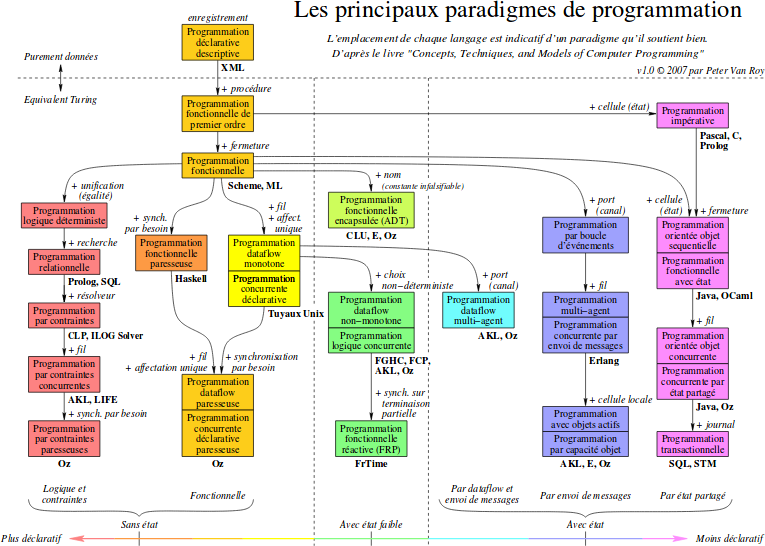
\includegraphics[scale=0.5]{graph.png}

\end{center}
\label{paradigme}
\caption{Les différents paradigmes de programmation}


\end{figure}
Source\cite{para}

\newpage
\begin{figure}[h]

\begin{center}

\begin{tabular}{|c|c|c|c|c|}

\cline{1-2}
\multicolumn{2}{|c|}{Classement} \\
\hline
2016 & 2015 & Langage & Utilisation & Changements \\
\hline 
1 & 2 & Java & 21,465\% & +5,94\% \\
\hline 
2 & 1 & C & 16,036\% & -0,67\% \\
\hline
3 & 4 & C++ & 6,914\% & +0,21\% \\
\hline
4 & 5 & C\# & 4,707\% & -0,34\% \\
\hline
5 & 8 & Python & 3,854\% & +1,24\% \\
\hline
6 & 6 & PHP & 2,706\% & -1,08\% \\
\hline
7 & 16 & Visual Basic .NET & 2,582\% & +1,51\% \\
\hline
8 & 7 & JavaScript & 2,565\% & -0,71\% \\
\hline
9 & 14 & Assembleur & 2,095\% & +0,92\% \\
\hline
10 & 15 & Ruby & 2,045\% & +0,92\% \\
\hline
11 & 9 & Perl & 1,841\% &  -0,42\% \\
\hline
12 & 20 & Delphi/Object Pascal & 1,786\% & +0,95\% \\
\hline
13 & 17 & Visual Basic & 1,684\% & +0,61\% \\
\hline
14 & 25 & Swift & 1,363\% & +0,62\% \\
\hline
15 & 11 & MATLAB & 1,228\% & -0,16\% \\
\hline
16 & 30 & Pascal & 1,194\% & +0,52\% \\
\hline
17 & 82 & Groovy & 1,182\% & +1,07\% \\
\hline
18 & 3 & Objective-C & 1,074\% & -5,88\% \\
\hline
19 & 18 & R & 1,054\% & +0,1\% \\
\hline
20 & 10 & PL/SQL & 1,016\% & -1\% \\
\hline
\multicolumn{5}{|c|}{...} \\
\hline

\end{tabular}

\end{center}
\label{ranking}
\caption{Classement des langages de programmation}


\end{figure}
Source\cite{rank}
\newpage
\begin{figure}[h]

\begin{center}

\begin{tikzpicture}
    \pie{21/Java, 16/C, 7/C++, 5/C\#, 4/Python, 3/PHP, 3/Visual Basic .NET, 3/JavaScript, 2/Assembleur, 39/Autres}
\end{tikzpicture}


\end{center}
\label{pie}
\caption{Utilisation des principaux langages de programmation}
\end{figure}
\newpage

\bibliographystyle{unsrt}
\bibliography{bibli}

\end{document}


